\section{\autoref{chapter-graphen}, \nameref{chapter-graphen}}

\subsection*{\ref{subsection-aufgaben-graphen-gerichtete-graphen} \nameref{subsection-aufgaben-graphen-gerichtete-graphen}}

\begin{enumerate}
	\item $G = (V, E)$ mit
\begin{align*}
	V & = \{v_1, v_2, v_3, v_4, v_5\} \\
	E & = \{(v_1, v_2), (v_2, v_3), (v_3, v_5), (v_1, v_5), (v_4, v_2), (v_5, v_4), (v_4, v_1), (v_1, v_3)\}
\end{align*}
	\item \autoref{figure-graph-aufgaben-gerichtete-graphen-sol-1} zeigt den Graphen grafisch.

\begin{figure}[ht]
\centering
\begin{minipage}{0.45\textwidth}
	\centering
	\begin{tikzpicture}
    \node[circle, fill, inner sep=2pt, label={north:$v_1$}] (v1) at (0,0) {};
    \node[circle, fill, inner sep=2pt, label={north:$v_2$}] (v2) at (2,0) {};
    \node[circle, fill, inner sep=2pt, label={south:$v_3$}] (v3) at (0,-2) {};
    \node[circle, fill, inner sep=2pt, label={south:$v_4$}] (v4) at (2,-2) {};
    \path[->, >=stealth', thick] (v1) edge (v2);
    \path[->, >=stealth', thick] (v2) edge (v3);
    \path[->, >=stealth', thick] (v3) edge (v4);
    \path[->, >=stealth', thick] (v4) edge (v1);
    \path[->, >=stealth', thick] (v2) edge (v4);
    \path[->, >=stealth', thick] (v1) edge (v3);
	\end{tikzpicture}
\caption{Graph mit vier Knoten und sechs Kanten.}
\label{figure-graph-aufgaben-gerichtete-graphen-sol-1}
\end{minipage}
\hfill
\begin{minipage}{0.45\textwidth}
	\centering
	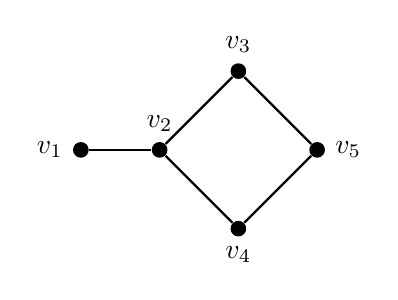
\begin{tikzpicture}
    \node[circle, fill, inner sep=2pt, label={west:$v_1$}] (v1) at (0,0) {};
    \node[circle, fill, inner sep=2pt, label={north:$v_2$}] (v2) at (1,0) {};
    \node[circle, fill, inner sep=2pt, label={north:$v_3$}] (v3) at (2,1) {};
    \node[circle, fill, inner sep=2pt, label={south:$v_4$}] (v4) at (2,-1) {};
    \node[circle, fill, inner sep=2pt, label={east:$v_5$}] (v5) at (3,0) {};
    \path (v1) edge[thick] (v2);
    \path (v2) edge[thick] (v4);
    \path (v2) edge[thick] (v3);
    \path (v3) edge[thick] (v5);
    \path (v4) edge[thick] (v5);
\end{tikzpicture}
\caption{Graph mit fünf Knoten und fünf Kanten.}
\label{figure-graph-aufgaben-ungerichtete-graphen-sol-1}
\end{minipage}

\end{figure}

\end{enumerate}

\subsection*{\ref{subsection-aufgaben-graphen-ungerichtete-graphen} \nameref{subsection-aufgaben-graphen-ungerichtete-graphen}}

\begin{enumerate}
	\item $G = \{V, E \}$ mit $V = \{v_1, v_2, v_3, v_4, v_5\}$ und
\begin{align*}
E & = \{\{v_1, v_2\}, \{v_1, v_3\}, \{v_1, v_4\}, \{v_1, v_5\}\}
\end{align*}
	
	\item \autoref{figure-graph-aufgaben-ungerichtete-graphen-sol-1} zeigt den Graphen grafisch.

\end{enumerate}

\subsection*{\ref{subsection-aufgaben-graphen-gewichtete-graphen} \nameref{subsection-aufgaben-graphen-gewichtete-graphen}}

\begin{enumerate}
	\item $G = (V, E, w)$ mit $V = \{v_1, v_2, v_3, v_4, v_5\}$ und
\begin{align*}
	E & =\{\{v_1, v_2\}, \{v_2, v_3\}, \{v_3, v_4\}, \{v_3, v_5\}, \{v_4, v_5\}, \{v_1, v_4\}\} \\
	w(\{v_1,v_2\}) & = 2 \\
	w(\{v_1,v_4\}) & = 5 \\
	w(\{v_2,v_3\}) & = 4 \\
	w(\{v_3,v_4\}) & = 6 \\
	w(\{v_3,v_5\}) & = 3 \\
	w(\{v_4,v_5\}) & = 1
\end{align*}
	
\item \autoref{figure-graph-aufgaben-gewichtete-graphen-sol-1} zeigt den Graphen grafisch. Es ist kein Distanzgraph, da der Graph negative Gewichte beinhaltet.

\begin{figure}[htb]
\centering
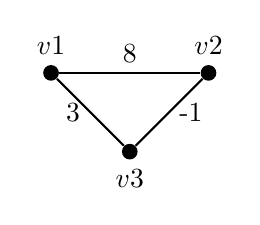
\begin{tikzpicture}
    \node[circle, fill, inner sep=2pt, label={north:$v1$}] (v1) at (0,0) {};
    \node[circle, fill, inner sep=2pt, label={north:$v2$}] (v2) at (2,0) {};
    \node[circle, fill, inner sep=2pt, label={south:$v3$}] (v3) at (1,-1) {};
    \path (v1) edge[thick] node[above] {8} (v2);
    \path (v2) edge[thick] node[right] {-1} (v3);
    \path (v1) edge[thick] node[left] {3} (v3);
\end{tikzpicture}
\caption{Graph mit drei Knoten und drei Kanten.}
\label{figure-graph-aufgaben-gewichtete-graphen-sol-1}
\end{figure}

\end{enumerate}